\documentclass[12pt]{article}
\usepackage{amsmath}
\usepackage{amssymb}
\usepackage[letterpaper,margin=0.85in,centering]{geometry}
\usepackage{fancyhdr}
\usepackage{enumerate}
\usepackage{lastpage}
\usepackage{multicol}
\usepackage{graphicx}

\reversemarginpar

\pagestyle{fancy}
\cfoot{}
\lhead{Math 2560}\chead{Worksheet \# 7}\rhead{Thursday 10\textsuperscript{th} March, 2016}
%\rfoot{Total: 10 points}
%\chead{{\bf Name:}}
\newcommand{\points}[1]{\marginpar{\hspace{24pt}[#1]}}
\newcommand{\skipline}{\vspace{12pt}}
%\renewcommand{\headrulewidth}{0in}
\headheight 30pt

\newcommand{\di}{\displaystyle}
\newcommand{\abs}[1]{\lvert #1\rvert}
\newcommand{\len}[1]{\lVert #1\rVert}
\renewcommand{\i}{\mathbf{i}}
\renewcommand{\j}{\mathbf{j}}
\renewcommand{\k}{\mathbf{k}}
\newcommand{\R}{\mathbb{R}}
\newcommand{\aaa}{\mathbf{a}}
\newcommand{\bbb}{\mathbf{b}}
\newcommand{\ccc}{\mathbf{c}}
\newcommand{\dotp}{\boldsymbol{\cdot}}
\newcommand{\bbm}{\begin{bmatrix}}
\newcommand{\ebm}{\end{bmatrix}}                   
                  
\begin{document}


%\author{Instructor: Sean Fitzpatrick}
\thispagestyle{fancy}
%\noindent{{\bf Name and student number:}}
The problems on this worksheet are for in-class practice during tutorial. You are free to collaborate and to ask for help. They don't count for course credit, but it's a good idea to make sure you know how to do everything before you leave tutorial -- similar problems may show up on a test or assignment.

\begin{enumerate}
 \item Evaluate the improper integral, or explain why it does not exist:
\begin{enumerate}
 \item $\di \int_0^\infty e^{4-3x}\,dx = \lim_{t\to \infty}\int_0^t e^{4-3x}\,dx = \lim_{t\to\infty}\frac{1}{3}(e^4-e^{4-3t})=e^4.$
 \item $\di \int_{-\infty}^\infty \frac{1}{4+x^2}\,dx = \lim_{s\to\infty}\int_{-s}^0\frac{1}{4+x^2}\,dx+\lim_{t\to\infty}\int_0^t\frac{1}{4+x^2}\,dx$.

Now we recall that $\di \int \frac{1}{4+x^2}\,dx = \frac{1}{2}\tan^{-1}(x/2)$, $\tan^{-1}(0)=0$, and $\lim_{x\to\pm\infty}\tan^{-1}x = \pm \frac{\pi}{2}$. It follows that $\lim_{x\to\infty}\tan^{-1}(\pm x/2) = \pm \frac{\pi}{2}$, since $x/2\to \infty$ if $x\to \infty$. Thus, we get
\[
 \int_{-\infty}^\infty \frac{1}{4+x^2}\,dx = -\frac{1}{2}\lim_{s\to \infty}\tan^{-1}(-s/2)+\frac{1}{2}\lim_{t\to\infty}\tan^{-1}(t/2) = \frac{\pi}{2}.
\]

 \item $\di \int_{-\infty}^\infty \frac{x}{1+x^2}\,dx = \int_{-\infty}^0 \frac{x}{1+x^2}\,dx + \int_0^\infty\frac{x}{1+x^2}\,dx$.

This integral diverges, since both of the two integrals on the right-hand side above diverge. Note that $\di \int\frac{1}{1+x^2}\,dx = \frac{1}{2}\ln(1+x^2)$, and as $x\to \pm\infty$, $\ln(1+x^2)\to\infty$.


 \item $\di \int_1^\infty\frac{\ln x}{x^2}\,dx$

\bigskip

Using integration by parts, $\di\int\frac{\ln x}{x^2}\,dx = -\frac{\ln x}{x}-\frac{1}{x}$. We thus have
\begin{align*}
 \int_1^\infty\frac{\ln x}{x^2}\,dx & = \lim_{t\to\infty}\int_1^t \frac{\ln x}{x^2}\,dx\\
& = \lim_{t\to\infty}\left(1-\frac{1}{t}-\frac{\ln t}{t}\right) = 1,
\end{align*}
where we have used the limits $\di\lim_{t\to\infty}\frac{1}{t} = 0$ and (using L'Hospital's rule for the indeterminate form $\infty/\infty$)
\[
 \lim_{t\to\infty}\frac{\ln t}{t} = \lim_{t\to\infty}\frac{1/t}{1} = 0.
\]



\end{enumerate}
 \item Find the area between the given curves:
\begin{enumerate}
 \item $y=x^2-3x+2$, and $y=-3x+3$

The sketches for both regions are given below. Here, the upper curve is $y=-3x+3$ and the lower curve is $y=x^2-3x+2$. The two curves intersect when $-3x+3=x^2-3x+2$, which gives us $x^2-1=0$, so $x=\pm 1$. Thus, we have
\[
 A = \int_{-1}^1[(3-3x)-(x^2-3x+2)]\,dx = \int_{-1}^1(1-x^2)\,dx = \frac{4}{3}.
\]


 \item $y=\sqrt{x}$, $y=-2x+3$, and $y=-\frac{1}{2}x$.

In this case, we can see from the sketch that it's necessary to break up the area into two regions. For $0\leq x\leq 1$, the upper curve is $y=\sqrt{x}$ and the lower curve is $y=-\frac{1}{2}x$, giving us the area
\[
 A_1 = \int_0^1\left(\sqrt{x}+\frac{1}{2}x\right)\,dx =\frac{11}{12}.
\]
For $1\leq x\leq 2$, the upper curve changes to $y=3-2x$, giving the area
\[
 A_2 = \int_1^2\left(3-2x+\frac{1}{2}x\right)\,dx = \frac{3}{4}.
\]
The total area is therefore $A=A_1+A_2 = \frac{5}{3}$.
\end{enumerate}

\begin{multicols}{2}
 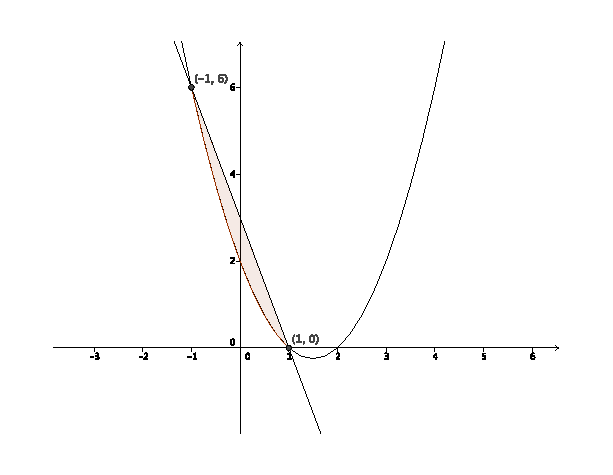
\includegraphics[width=0.9\columnwidth]{WS7-2a}

 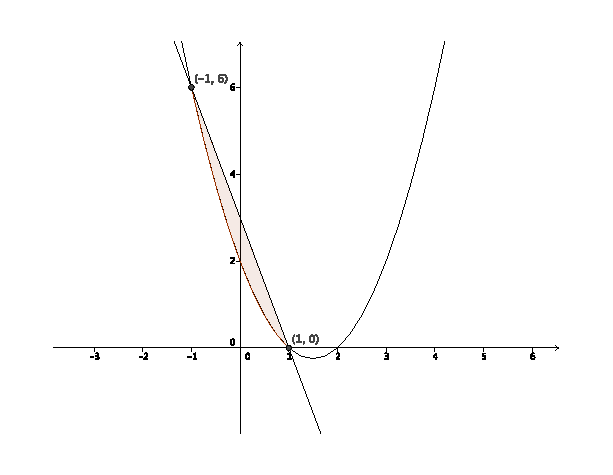
\includegraphics[width=0.9\columnwidth]{WS7-2a}
\end{multicols}

\item Find the volume of the solid of revolution:
\begin{enumerate}
 \item Generated by revolving the region bounded by $y=x^2-2x+2$ and $y=2x-1$ about the $x$-axis.

\begin{center}
 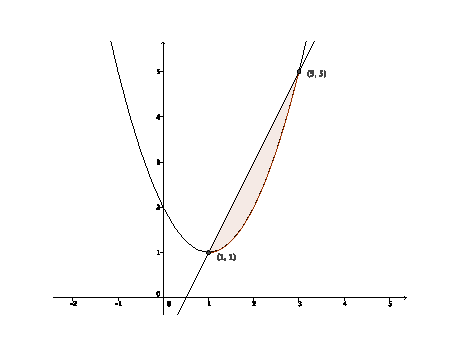
\includegraphics[width=0.5\textwidth]{WS7-3a}
\end{center}

The region for parts (a) and (b) is shown above. Since we're revolving about the $x$-axis for part (a), the washer method is more convenient, as it involves an integral with respect to $x$. (The shell method would require us to solve for $x$ as a function of $y$.)

The outer radius for our washer is given by the value of the $y$-coordinate of the curve that is furthest from the $x$-axis, so we have $r_{out} = 2x-1$. The inner radius is given by the closer of the two curves, so $r_{in} = x^2-2x+2$. Putting these into the formula for volume by washers gives us
\begin{align*}
 V & = \pi\int_1^3 \left[(2x-1)^2-(x^2-2x+2)^2\right]\,dx\\
& = \pi\int_1^3 (-x^4+4x^3-4x^2+4x-3)\,dx = \frac{104\pi}{15}.
\end{align*}
(I don't promise that I avoided computational errors on this one!)


 \item Generated by revolving the region bounded by $y=x^2-2x+2$ and $y=2x-1$ about the line $y=1$.

\bigskip

Since the axis of rotation is vertical this time, we want to use shells in order to integrate with respect to $x$. The radius of each shell is $r(x)=x-1$, and the height is given by the difference in the $y$-values of the two curves: $h(x)=(2x-1)-(x^2-2x+2) = -x^2+4x-3$. Thus, we have
\[
 V = 2\pi\int_1^3 (x-1)(-x^2+4x-3)\,dx = \frac{8\pi}{3}.
\]

 \item Generated by revolving the triangle with vertices $(1,1), (1,2)$, and $(2,1)$ about the $y$-axis.

\begin{center}
 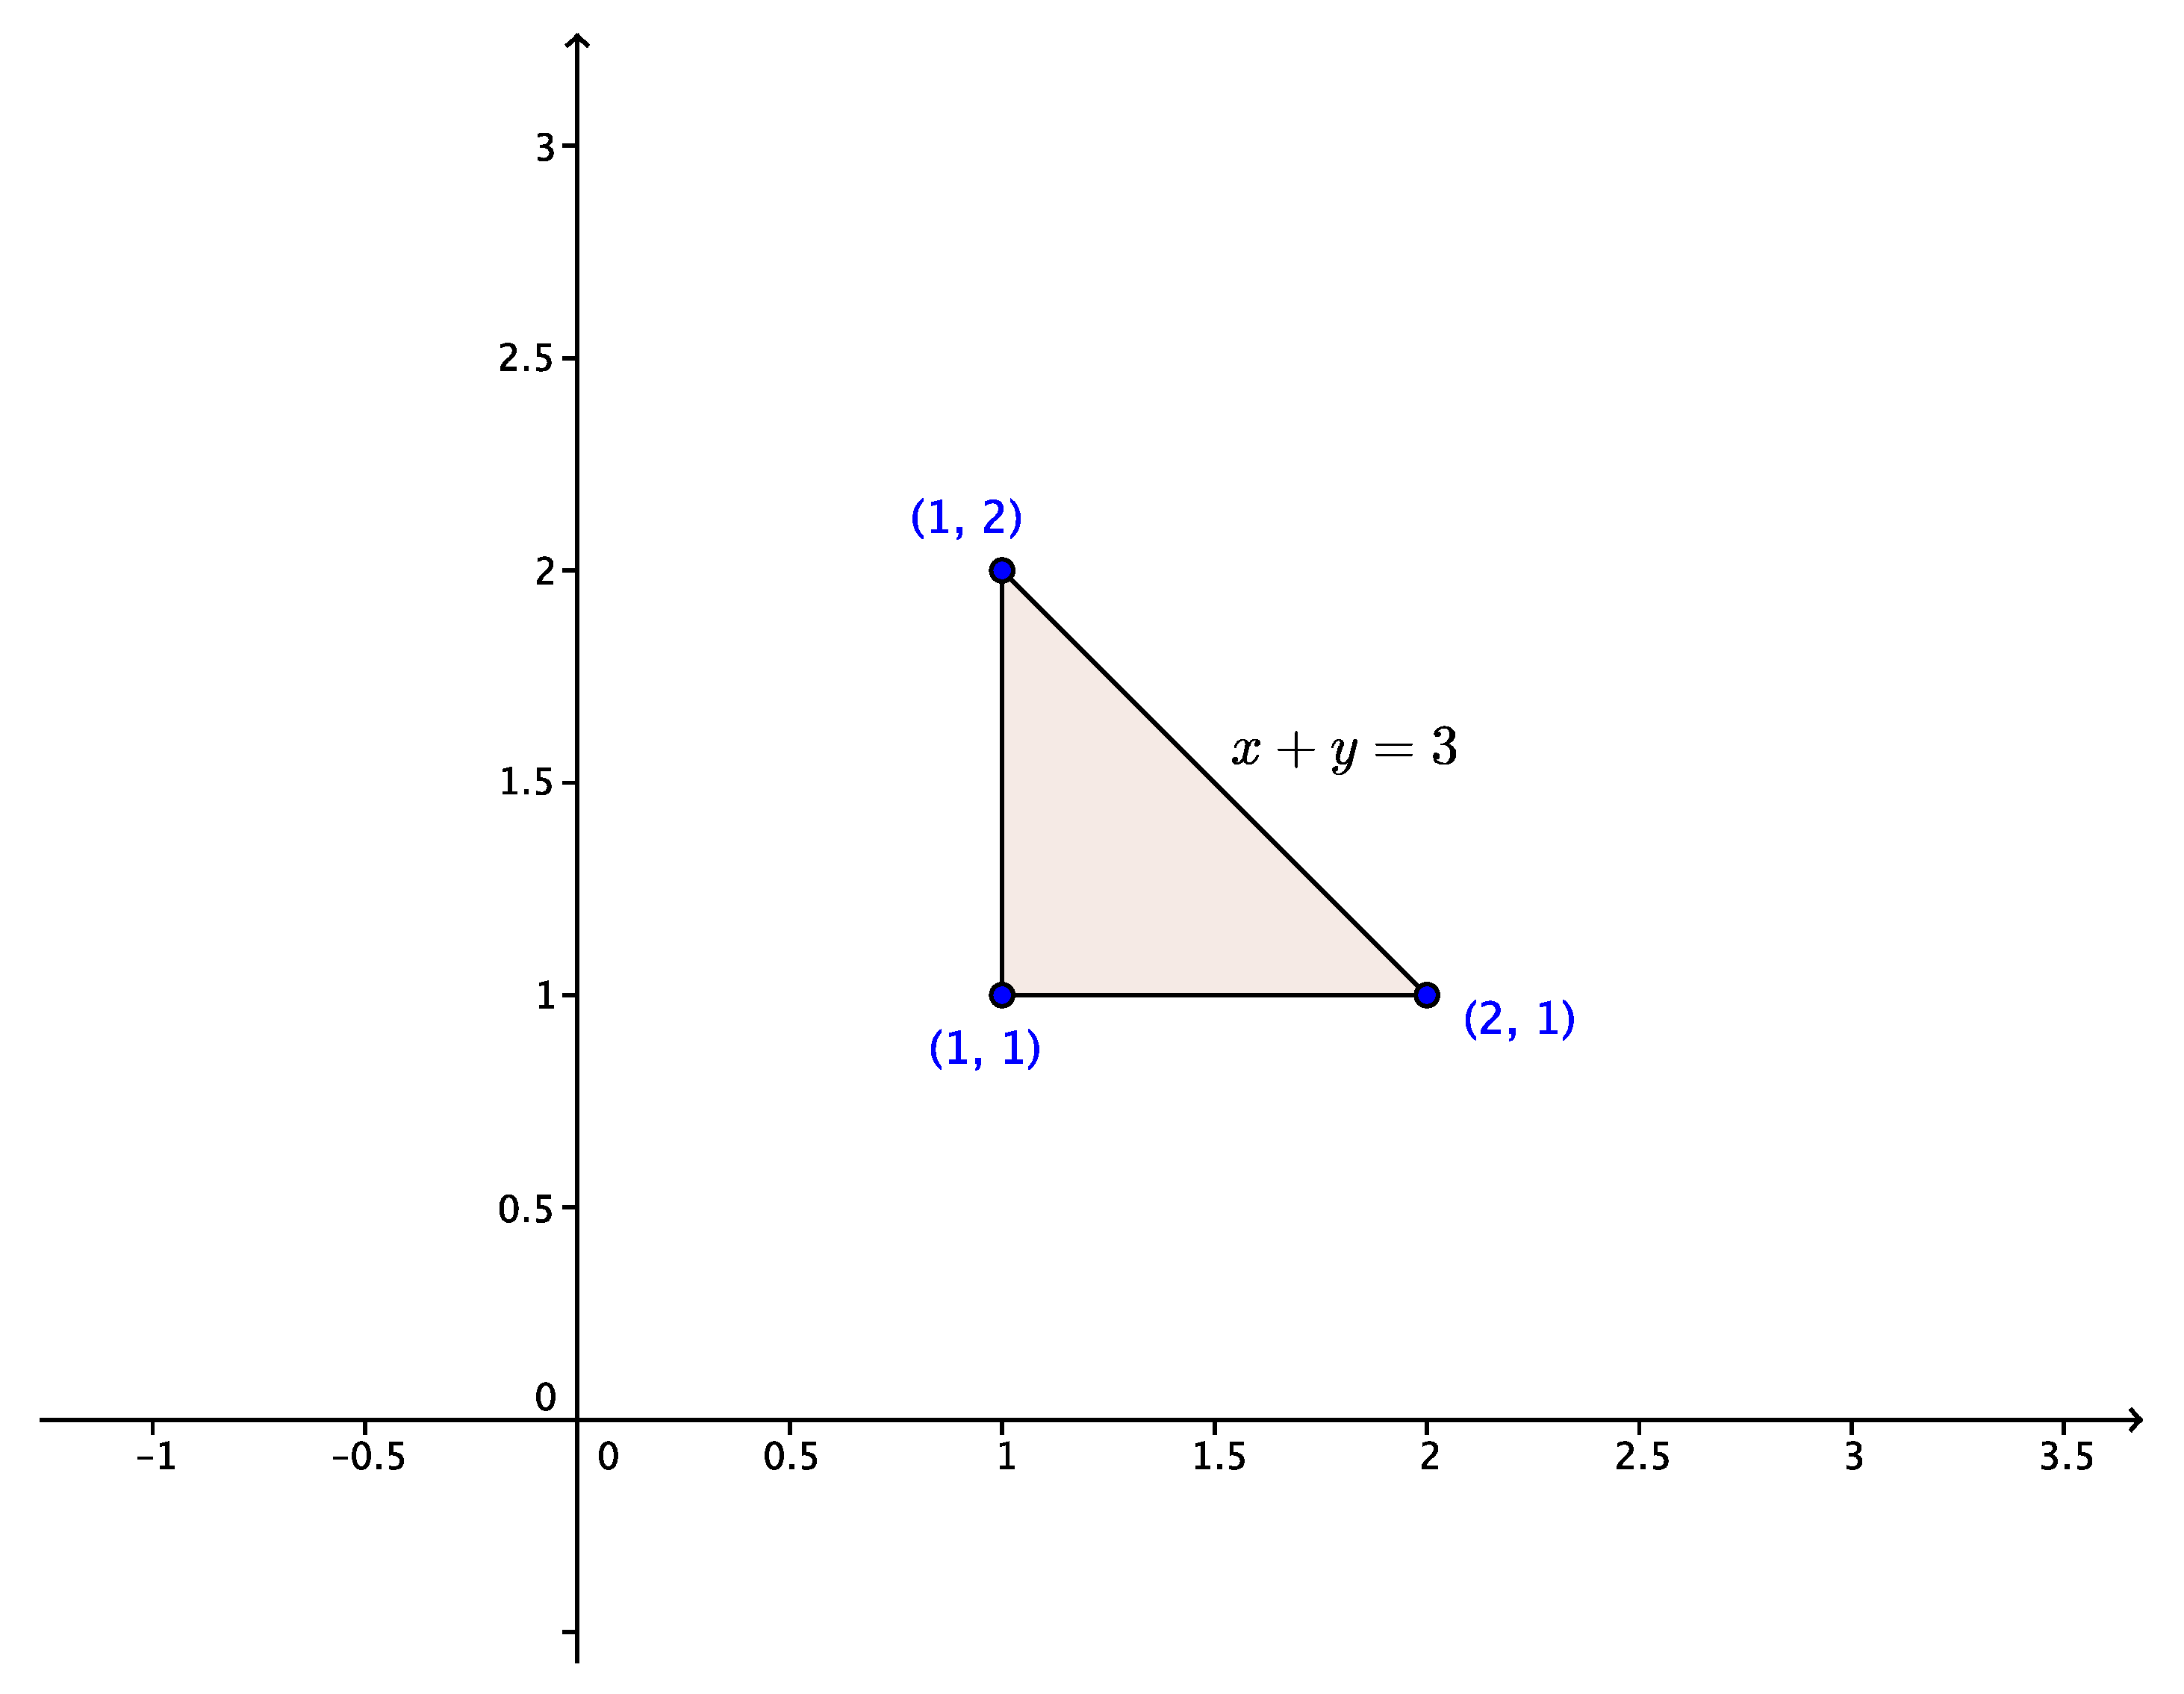
\includegraphics[width=0.5\textwidth]{WS7-3c}
\end{center}

The region to be revolved is shown above. If we choose to use washers, then we write the equation of the hypotenuse of the triangle as $x=3-y$, since we integrate with respect to $y$ for a vertical axis. The inner radius is simply 1 (the vertical side of the triangle), so we have (as seen in tutorial)
\[
 V = \pi\int_1^2[(3-y)^2-1]\,dy = \frac{4\pi}{3}.
\]
If we choose to use shells instead, then the radius of the shell is $x$, and the height is $(3-x)-1 = 2-x$, giving us
\[
 V = 2\pi\int_1^2 x(2-x)\,dx = \frac{4\pi}{3}.
\]



 \item Generated by revolving the triangle with vertices $(1,1), (1,2)$, and $(2,1)$ about the $x$-axis.

\bigskip

The symmetry of the region tells us that the answer here will be the same as the one given above. The only difference is that the washer method will be an integral with respect to $x$, and the shell method will be an integral with respect to $y$.
\end{enumerate}
\item Find the length of the curve $y=2x^{3/2}-\dfrac{1}{\sqrt{6}}\sqrt{x}$, for $0\leq x\leq 9$.

\bigskip

OK, typo on this one. It should have been $y=2x^{3/2}-\dfrac{1}{6}\sqrt{x}$. Otherwise it's a big mess. With the typo fixed,
\[
 1+(y')^2 = 1+\left(3\sqrt{x}-\frac{1}{12\sqrt{x}}\right)^2 = 1+\left(\frac{36x-1}{12\sqrt{x}}\right)^2 = \left(\frac{36x+1}{12\sqrt{x}}\right)^2.
\]
Thus, the length is
\[
 L = \int_0^9\sqrt{1+(y')^2}\,dx = \int_0^9 \left(3x^{1/2}+\frac{1}{12}x^{-1/2}\right)\,dx = \frac{107}{2}.
\]

\item Find the area of the surface generated by revolving the the curve $y=x^2$, for $0\leq x\leq 1$, about the $y$-axis.

\bigskip

Since we're revolving about the $y$-axis, we use the formula $S = 2\pi\int_a^b x\sqrt{1+(y')^2}\,dy$, giving us
\[
 S = 2\pi\int_0^1 x\sqrt{1+(2x)^2}\,dx = \frac{\pi}{6}(5\sqrt{5}-1).
\]

\item Find the area enclosed by the following regions:
\begin{enumerate}
 \item The region above the $x$-axis and below the spiral $r=\theta$, for $0\leq \theta \leq \pi$.

We have $A = \di\frac{1}{2}\int_0^\pi \theta^2\,d\theta = \frac{\pi^3}{6}$.

 \item The region given by the part of the first quadrant inside the curve $r=1+\sin\theta$.

We have $A = \frac{1}{2}\int_0^{\pi/2}(1+\sin\theta)^2\,d\theta = 1+\frac{3\pi}{8}$.

 \item One loop of the curve $r=\sin 4\theta$.

We note that $r=0$ for $\theta = 0, \pi/4, \pi/2, 3\pi/4, \ldots$, so one loop is given by taking $0\leq \theta\leq \pi/4$. Thus, we have
\[
 A = \frac{1}{2}\int_0^{\pi/4}\sin^2(4\theta)\,d\theta = \frac{1}{4}\int_0^{\pi/4}(1-\cos(8\theta))\,d\theta  = \frac{\pi}{16}.
\]

 \item The inner loop of the curve $r=1+2\sin\theta$.

We note that $r=0$ if $\sin\theta = -\dfrac{1}{2}$, which gives us $\theta = 7\pi/6$ or $\theta = 11\pi/6$. Thus,
\[
 A = \frac{1}{2}\int_{7\pi/6}^{11\pi/6}(1+2\sin\theta)^2\,d\theta = \pi-3\sqrt{3}/2.
\]

\end{enumerate}


Diagrams for problem 6:
\begin{multicols}{2}
 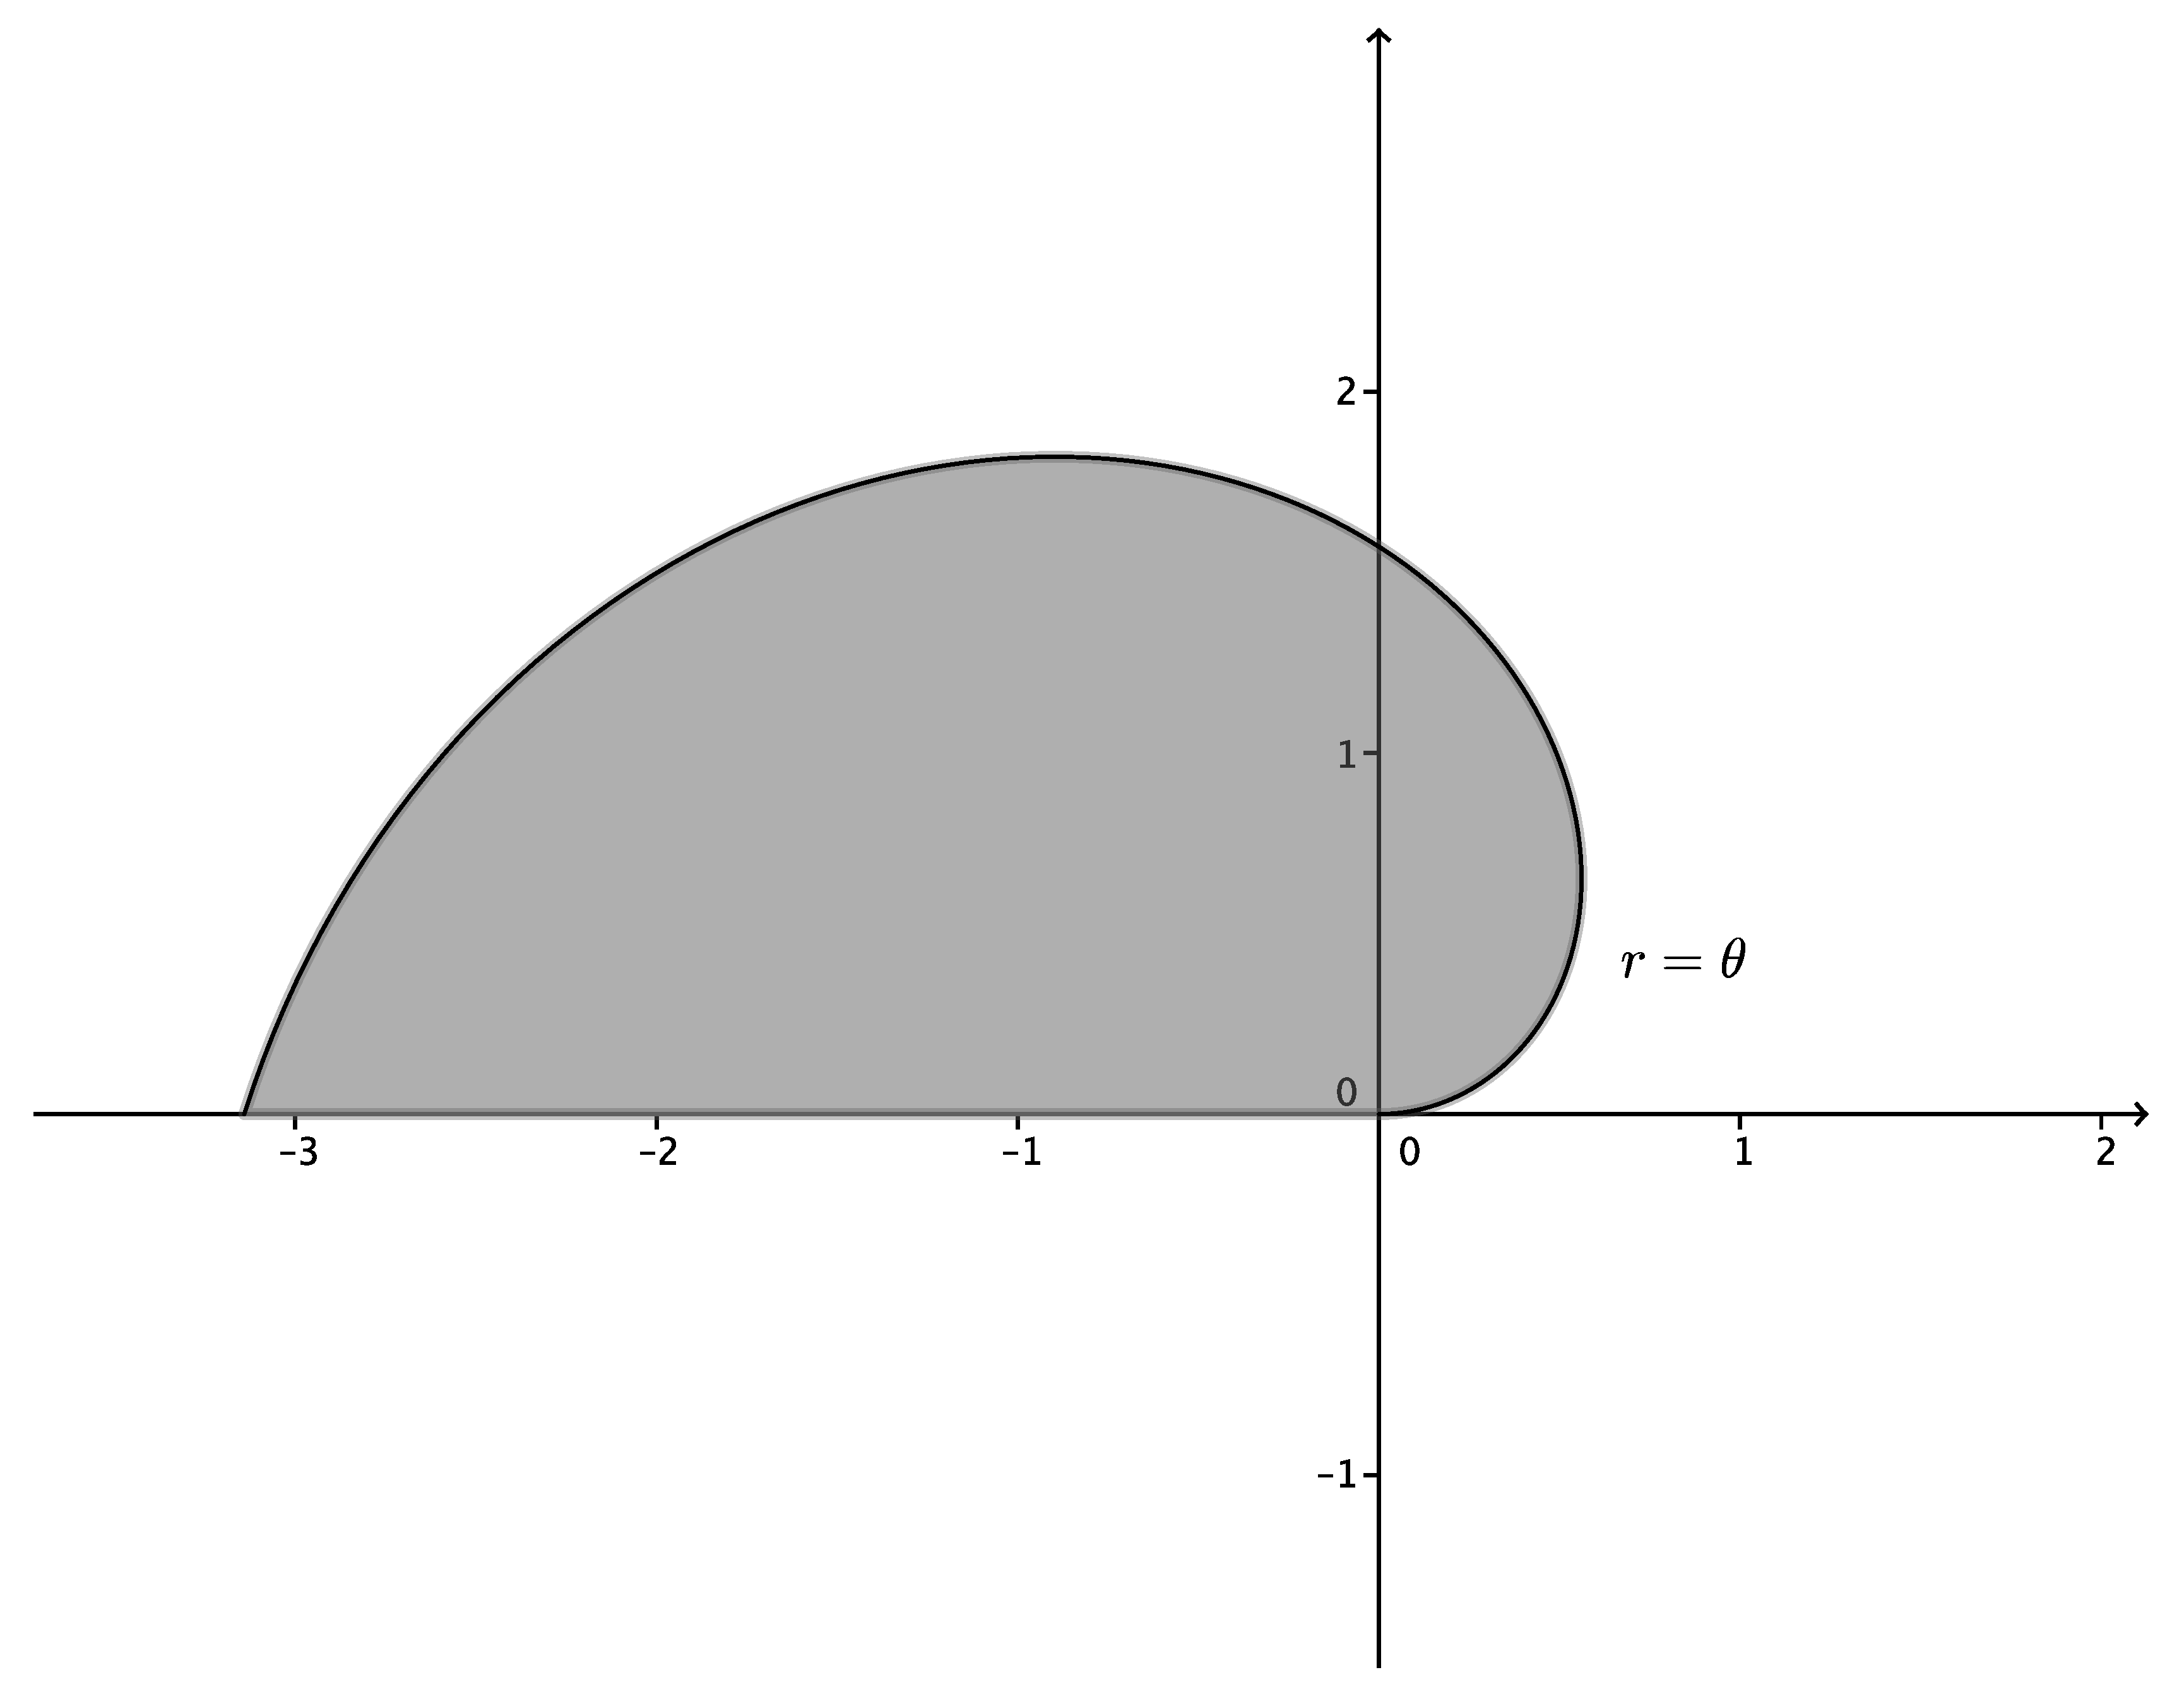
\includegraphics[width=0.9\columnwidth]{WS7-6a}

 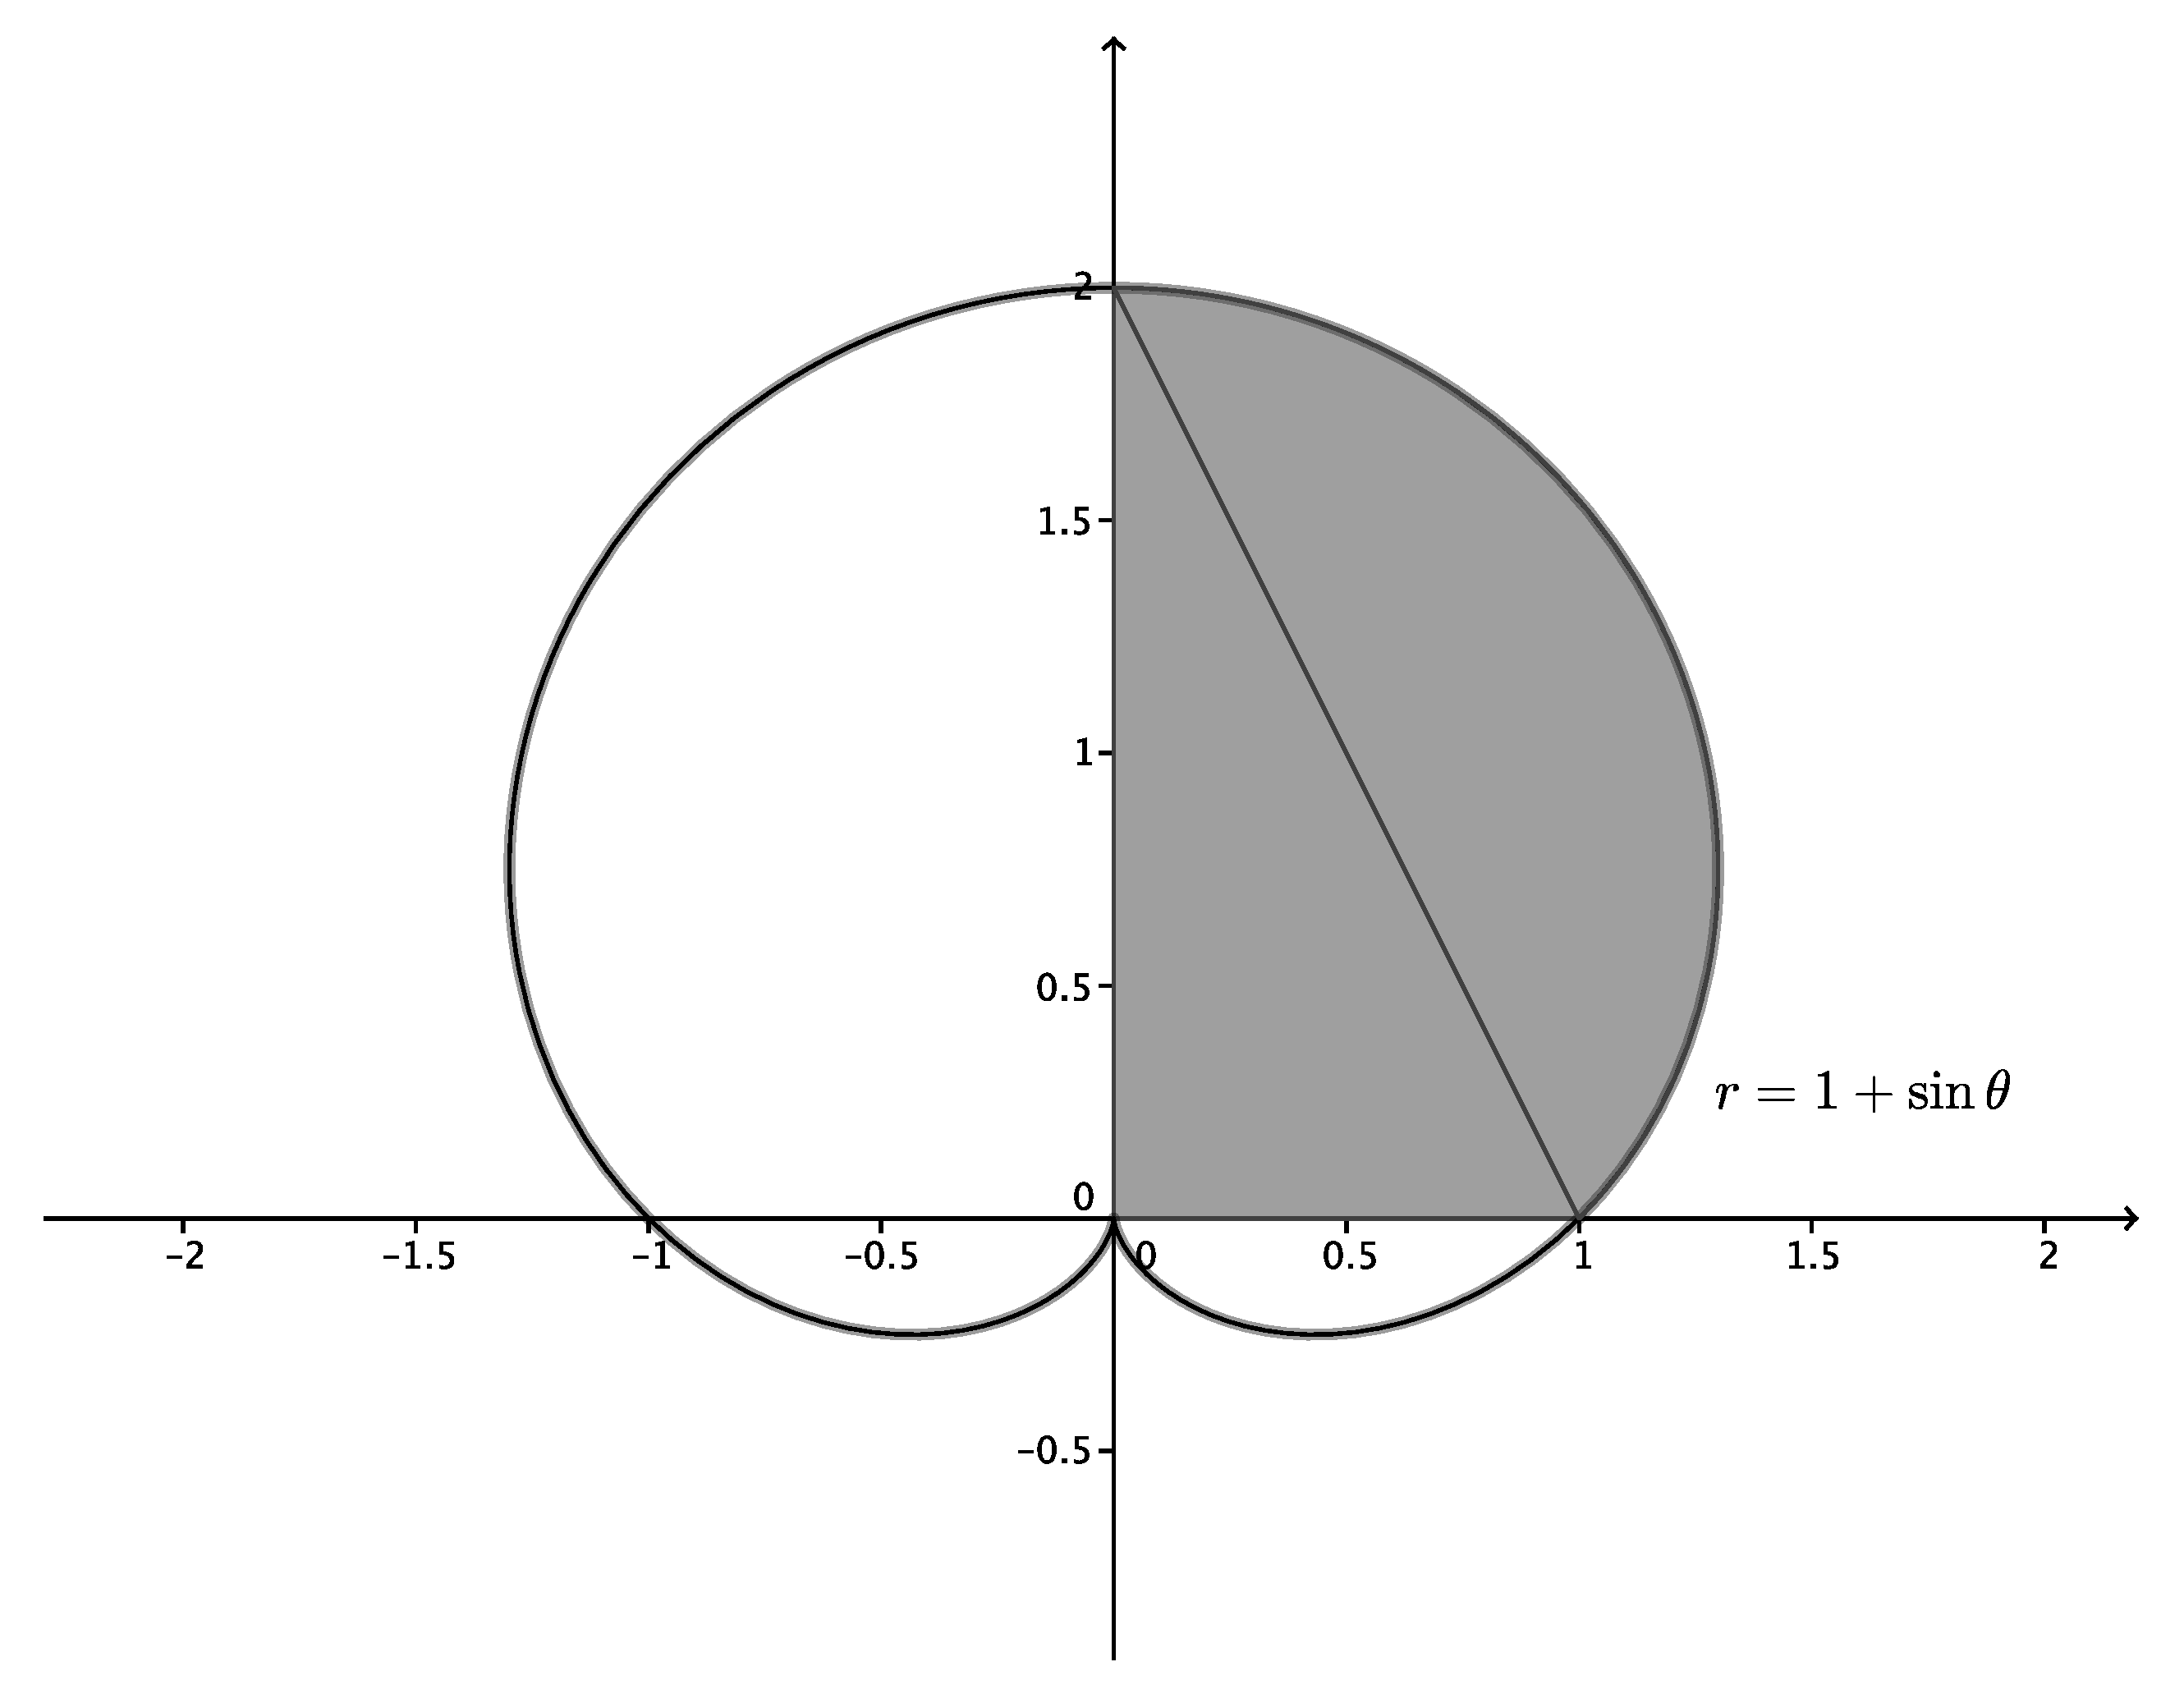
\includegraphics[width=0.9\columnwidth]{WS7-6b}

 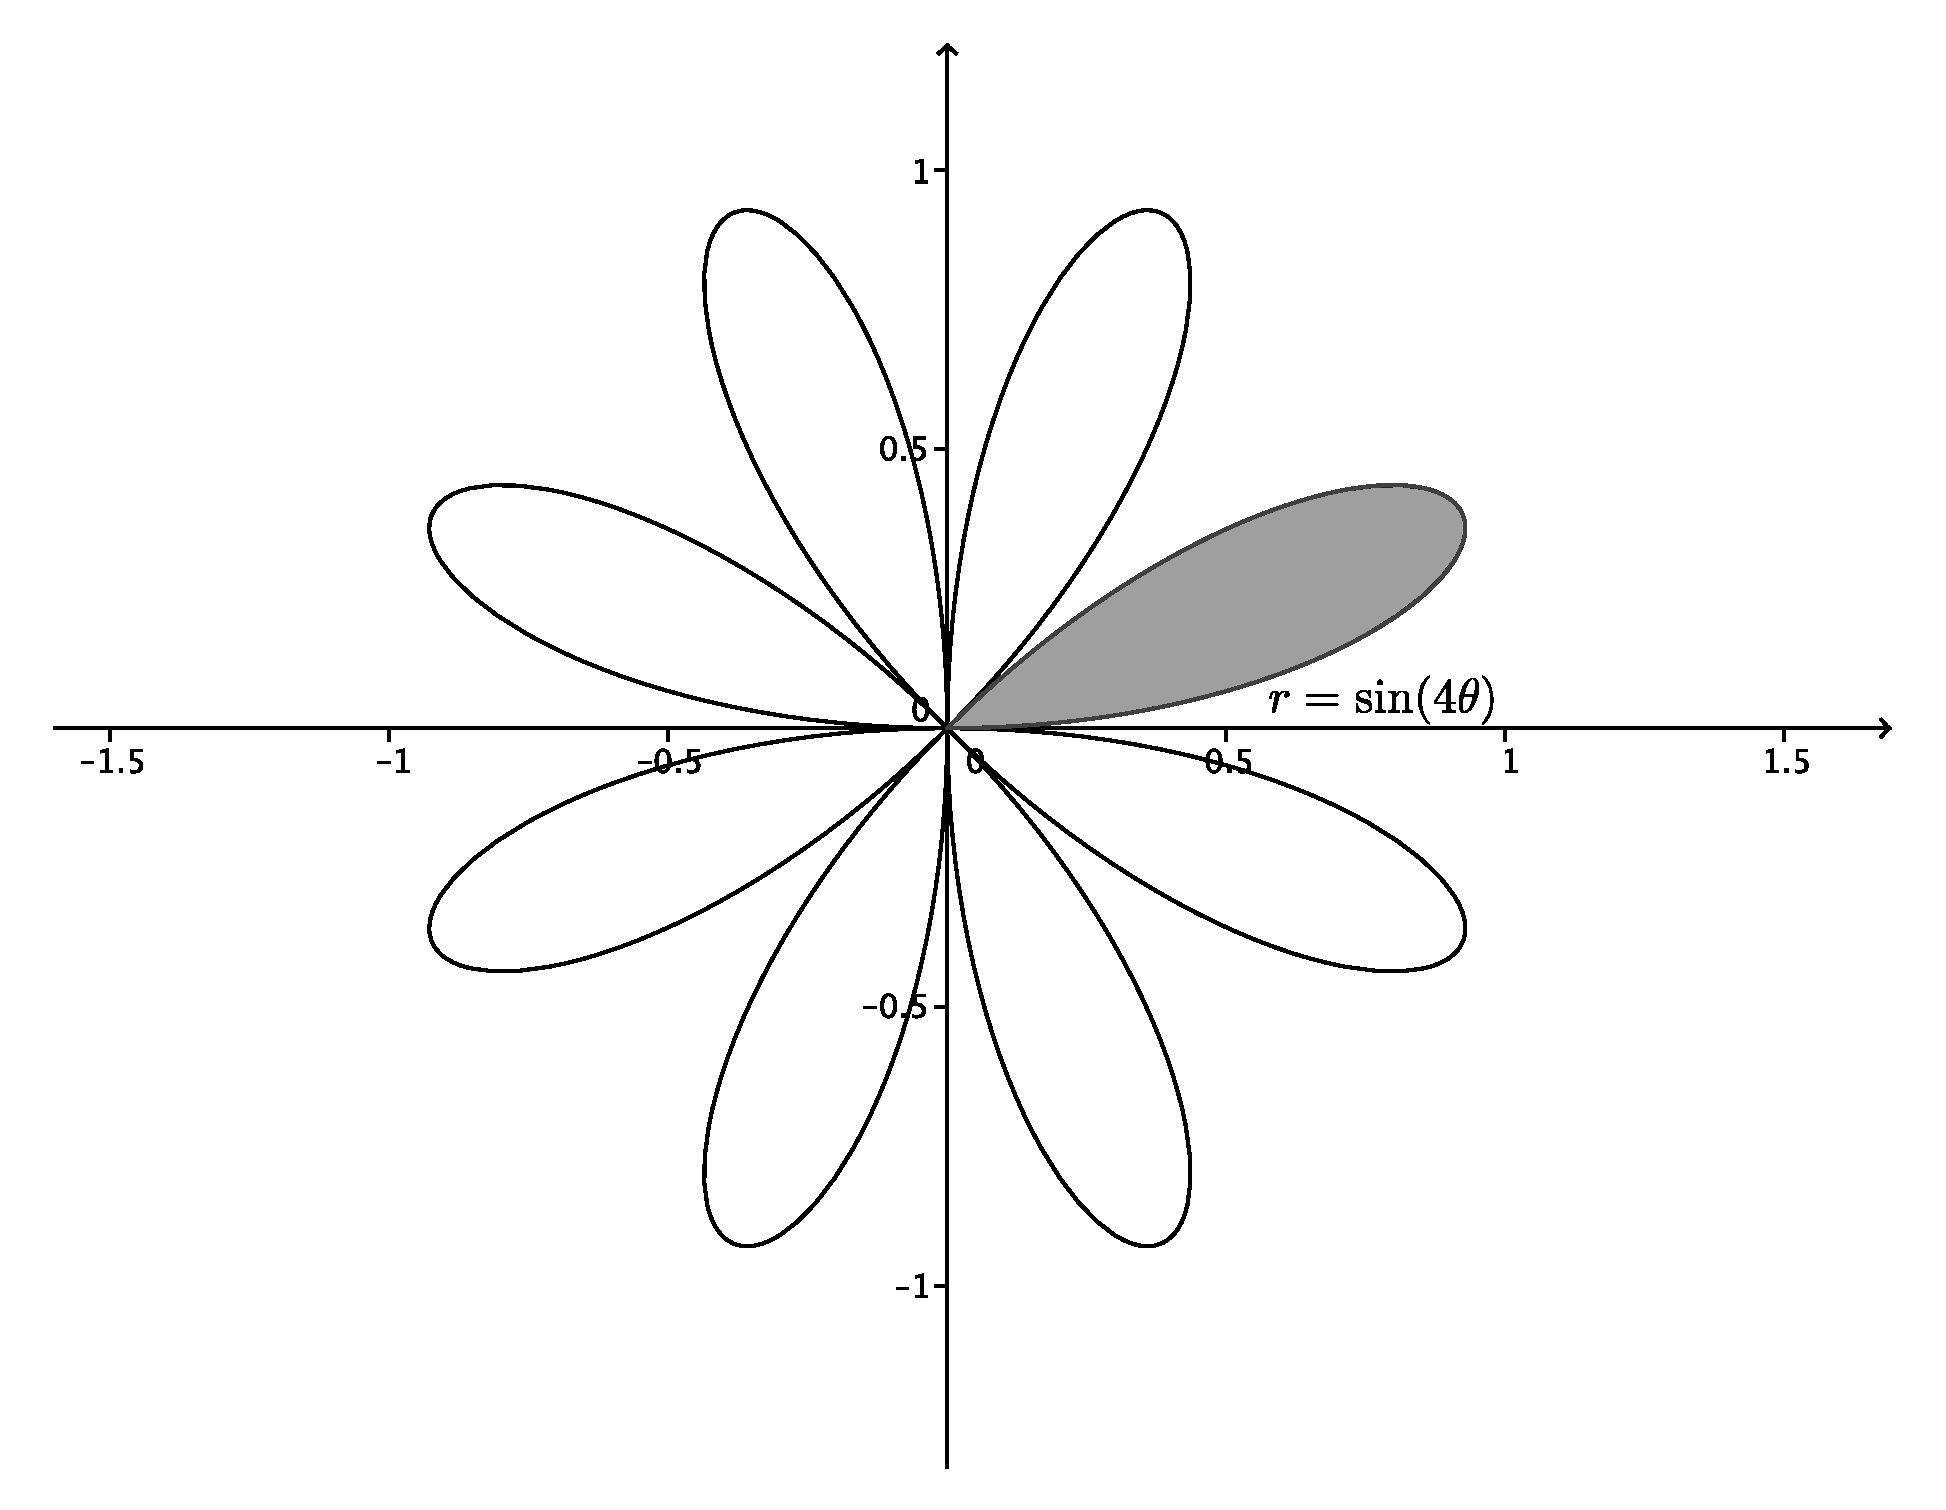
\includegraphics[width=0.9\columnwidth]{WS7-6c}

 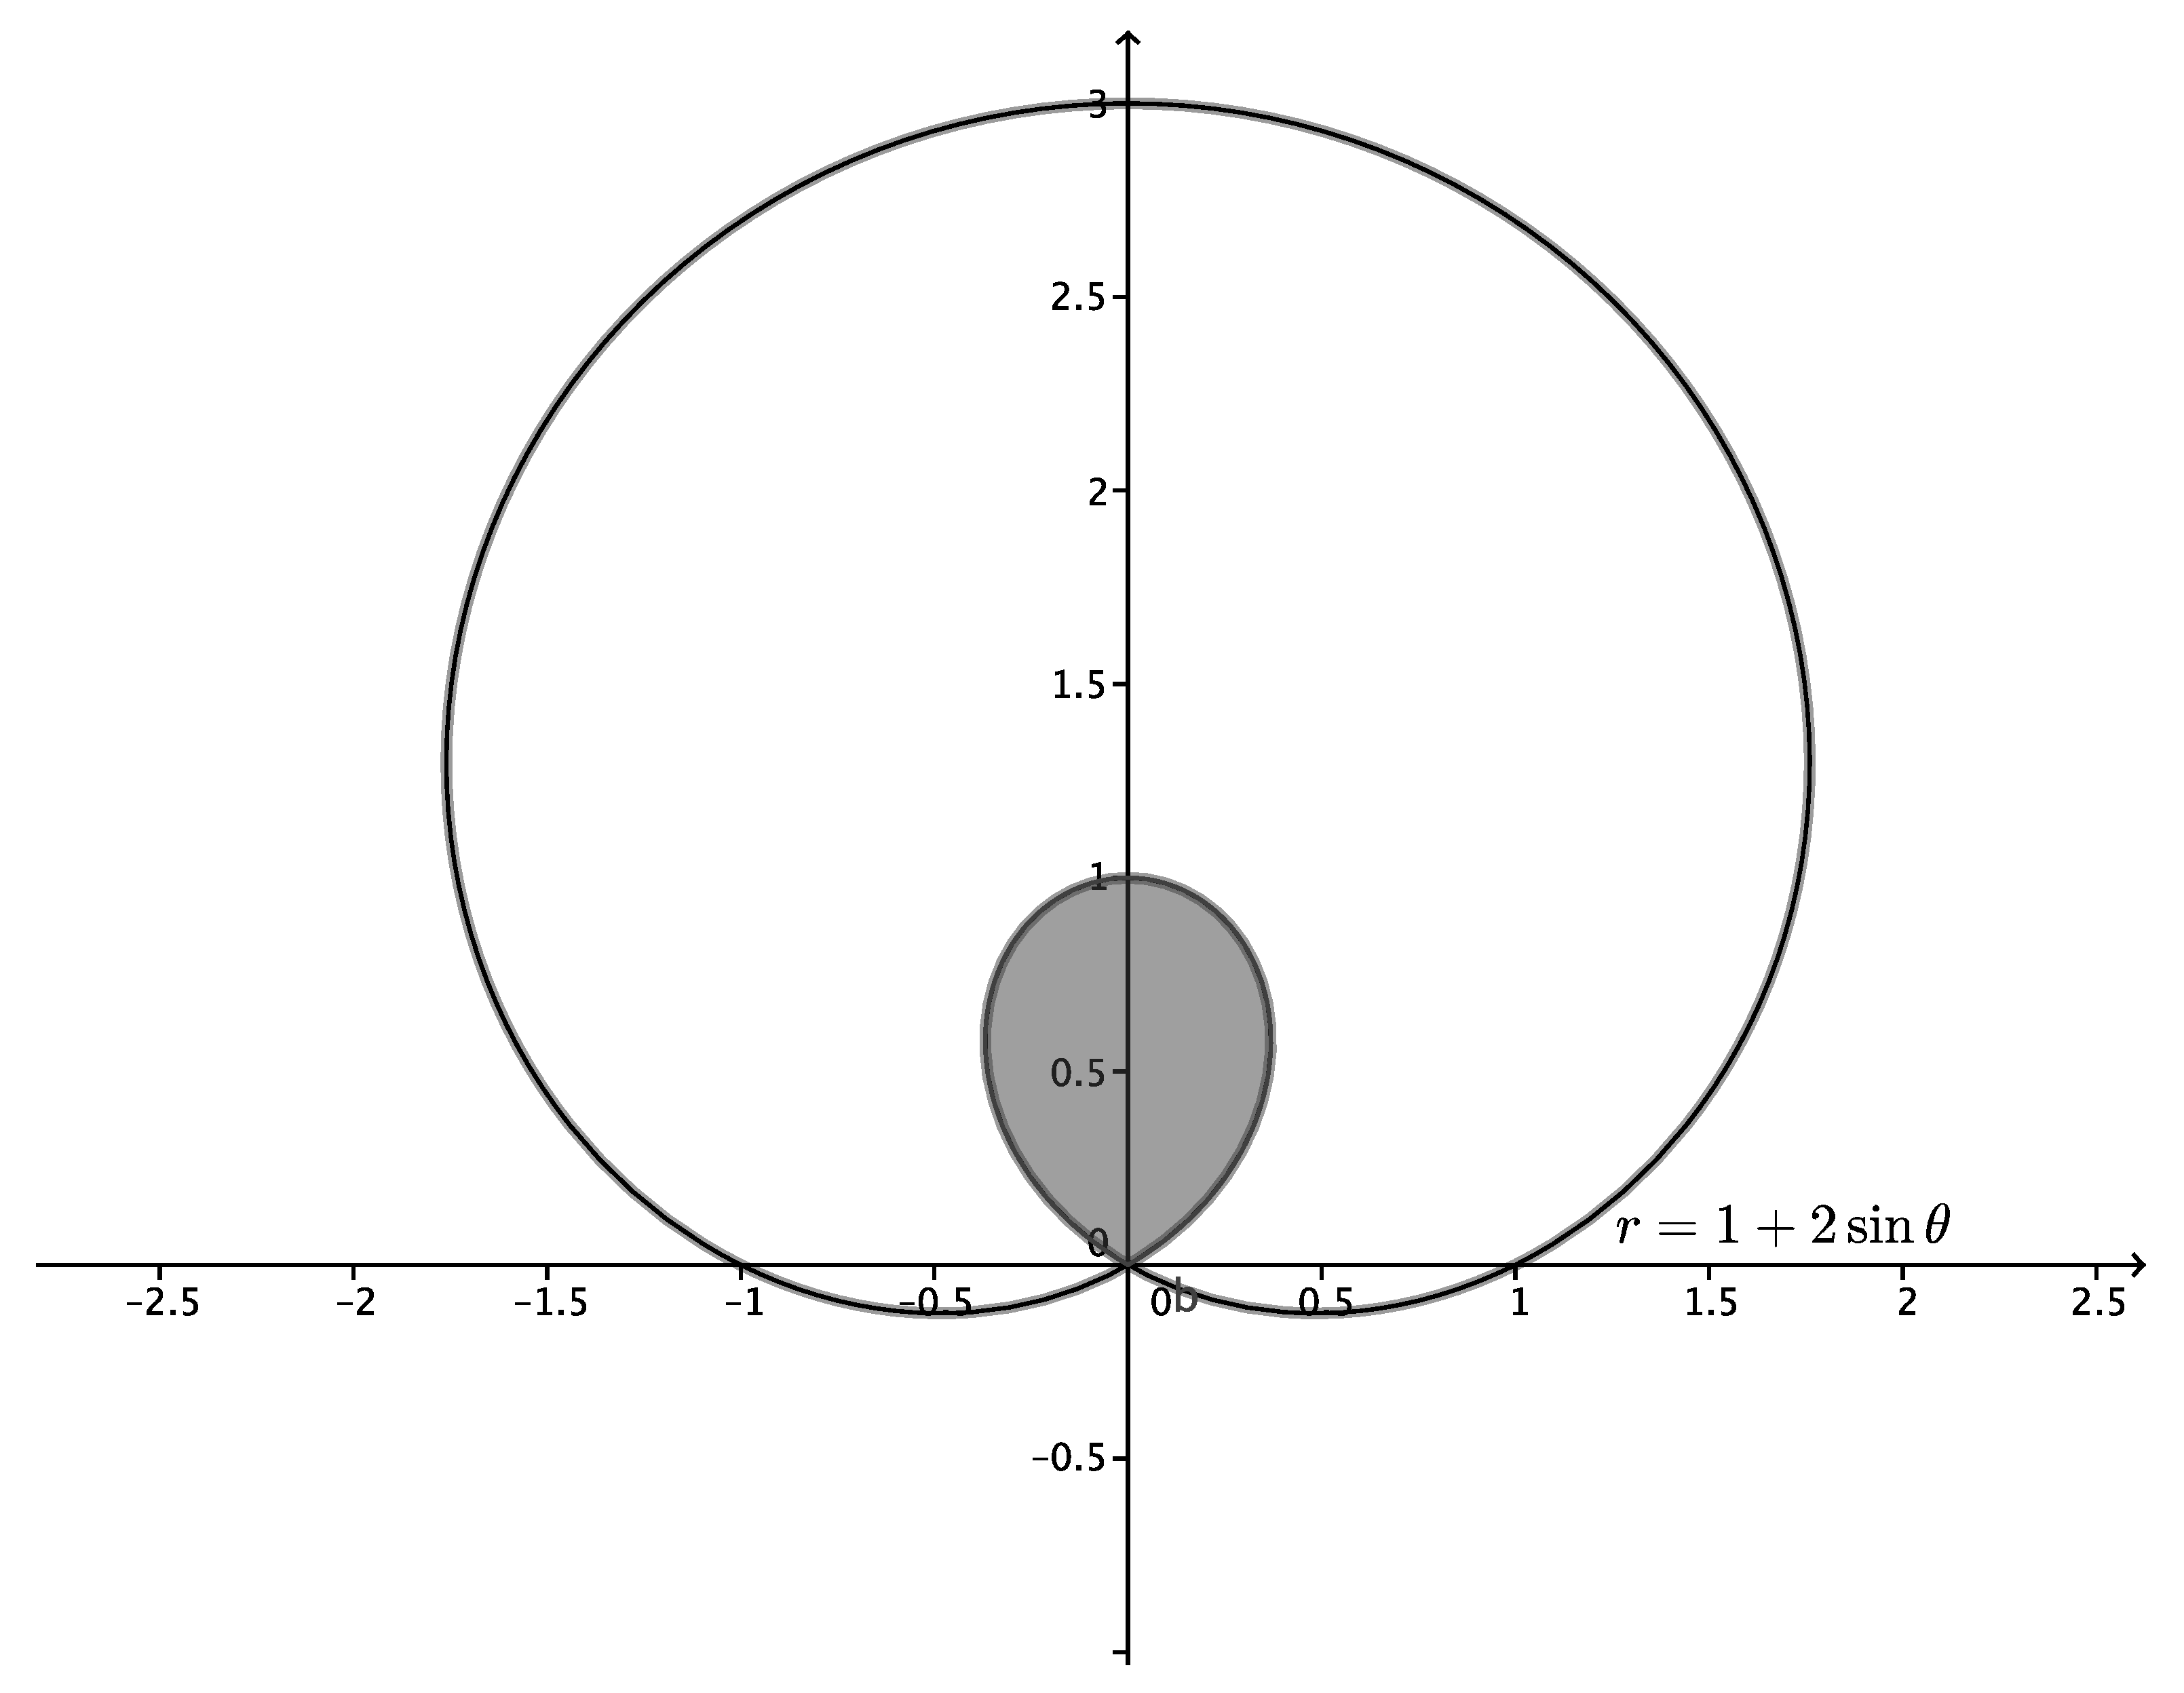
\includegraphics[width=0.9\columnwidth]{WS7-6d}

\end{multicols}


\end{enumerate}





\end{document}